\section{Hệ thống đề xuất}

\subsection{Mô tả hệ thống}
Trên cơ sở phân tích và đánh giá các giải pháp hỗ trợ du lịch hiện có ở Chương 4, chương này đề xuất Hệ thống Gợi ý Hành trình Du lịch Thông minh TravelEZ nhằm giải quyết các hạn chế đã được chỉ ra. Hệ thống được cấu thành từ các nhóm chức năng chính, mỗi nhóm đảm nhiệm một vai trò chuyên biệt để hiện thực hóa mục tiêu xây dựng một nền tảng du lịch toàn diện — từ việc tạo ra các gợi ý cá nhân hóa sâu sắc, thúc đẩy tương tác cộng đồng, cho đến việc cung cấp công cụ hỗ trợ cho các nhà cung cấp dịch vụ.

Hệ thống bao gồm 8 module chính sau:

% --- HÌNH ẢNH TỔNG QUAN ĐƯỢC ĐẶT NGAY TRƯỚC DANH SÁCH MODULE ---
\begin{figure}[H]
    \centering
    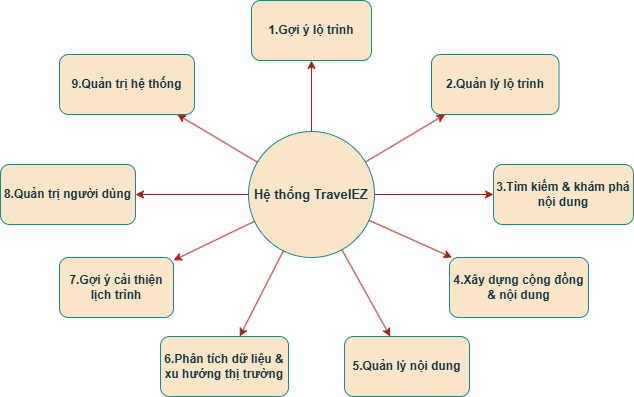
\includegraphics[width=0.9\textwidth]{Images/5 Hệ thống đề xuất/System Overview.png} 
    \caption{Sơ đồ tổng quan các thành phần chính của hệ thống TravelEZ.}
    \label{fig:system_overview}
\end{figure}

% --- MÔ TẢ CHI TIẾT CÁC MODULE ---
\begin{enumerate}
    \item \textbf{MD-01 Gợi ý lộ trình:} Tiếp nhận yêu cầu lập kế hoạch (điểm đến, thời gian, ngân sách, sở thích), xử lý và đề xuất kế hoạch lộ trình chi tiết (theo ngày/khung giờ). Người dùng tùy chỉnh lộ trình (thêm/xoá/sắp xếp lại điểm đến, điều chỉnh thời gian), lưu trữ và quản lý các phiên bản kế hoạch.

    \item \textbf{MD-02 Quản lý lộ trình:} Người dùng có thể chia sẻ kế hoạch với bạn bè và tích hợp lộ trình với Google Calendar.

    \item \textbf{MD-03 Tìm kiếm và khám phá:} Cung cấp chức năng tìm kiếm thông tin (địa điểm, dịch vụ, bài viết), lọc kết quả nâng cao (khu vực, loại hình, đánh giá, độ phổ biến), hiển thị kết quả trên bản đồ tương tác, lưu (bookmark) nội dung yêu thích vào bộ sưu tập cá nhân. 

    \item \textbf{MD-04 Xây dựng cộng đồng và nội dung:} Cho phép đăng tải bài viết, đánh giá (review) và xếp hạng (rating) cho dịch vụ, tương tác (bình luận, theo dõi), quản lý hồ sơ cá nhân và các nội dung đã đóng góp.
    
    \item \textbf{MD-05 Quản lý nội dung:} Cung cấp giao diện cho quản trị viên quản lý nội dung đăng tải, kiểm duyệt, xử lý tài khoản vi phạm, tiếp nhận và xử lý báo cáo (report) từ người dùng.

    \item \textbf{MD-06 Phân tích dữ liệu và xu hướng thị trường:} Cung cấp dashboard (cho nhà cung cấp) hiển thị các số liệu thống kê, trực quan hóa dữ liệu và trình bày các xu hướng thịnh hành (điểm đến, chủ đề tìm kiếm).

    \item \textbf{MD-07 Gợi ý cải thiện lịch trình:} Phân tích các lộ trình/tour hiện có của nhà cung cấp dịch vụ, cung cấp các gợi ý điều chỉnh cụ thể.

    \item \textbf{MD-08 Quản trị hệ thống \& người dùng:} Xử lý xác thực người dùng, quản lý hồ sơ người dùng, phân quyền truy cập (admin, provider, tourist), quản
    
\end{enumerate}


\subsection{Mô tả người dùng}
\label{sec:mo_ta_nguoi_dung}
Hệ thống phân chia người dùng thành hai nhóm tài khoản chính: Người dùng cuối (END\_USERS) và Quản trị viên (ADMINS). Mỗi tài khoản được gán một vai trò (ROLE) cụ thể để phân định rõ ràng quyền hạn và chức năng.

\begin{enumerate}

    \item \textbf{Khách du lịch (TRAVELER):} Là vai trò cốt lõi của hệ thống. Họ có đầy đủ quyền truy cập vào các tính năng lập kế hoạch (tạo/quản lý lịch trình cá nhân) và các tính năng xã hội như viết blog, đánh giá (review), kết bạn, theo dõi và tương tác với cộng đồng.
        
       \item \textbf{Nhà cung cấp (PROVIDER):} Là một tài khoản đã đăng ký, tập trung vào việc sử dụng các công cụ phân tích. Họ có quyền truy cập vào các dashboard thống kê xu hướng du lịch (từ Module 6) và sử dụng công cụ AI để phân tích, cải thiện lịch trình (từ Module 7). Họ không có quyền tạo hay chỉnh sửa dịch vụ trên nền tảng.

    \item \textbf{Quản trị viên (ADMINS):} Là nhóm tài khoản chịu trách nhiệm vận hành, duy trì và kiểm soát hệ thống. 
\end{enumerate}

\subsection{Yêu cầu chức năng}
\Needspace{12\baselineskip}
% \begin{longtable}{|p{2.5cm}|p{2.5cm}|p{3.5cm}|p{6.5cm}|}

% % --- ĐỊNH NGHĨA TIÊU ĐỀ BẢNG (LẶP LẠI TRÊN MỖI TRANG) ---
% \hline
% \textbf{Người dùng} & \textbf{Mã chức năng} & \textbf{Tên chức năng} & \textbf{Mô tả ngắn} \\
% \hline
% \endfirsthead % Tiêu đề này chỉ xuất hiện ở trang đầu tiên.

% % \hline
% % \multicolumn{4}{|l|}{\textit{... tiếp theo}} \\
% \hline
% % \textbf{Người dùng} & \textbf{Mã chức năng} & \textbf{Tên chức năng} & \textbf{Mô tả ngắn} \\
% % \hline
% \endhead % Tiêu đề này sẽ lặp lại ở các trang tiếp theo.

% % --- ĐỊNH NGHĨA CHÂN TRANG BẢNG ---
% \hline
% % \multicolumn{4}{r|}{\textit{(Còn tiếp)}} \\
% \endfoot % Chân trang này xuất hiện ở cuối các trang bị ngắt.

% % \hline
% \endlastfoot % Chân trang này chỉ xuất hiện ở cuối cùng của bảng.


% % --- NỘI DUNG BẢNG ---
% \multicolumn{4}{|l|}{\textbf{US-01: Khách (Guest)}} \\
% \hline
% % Để trống cột đầu tiên để duy trì cấu trúc và sự phân cấp
%  & FR-GST-01 & Xem review & Hiển thị các đánh giá (review) công khai về địa điểm, dịch vụ. \\
% \cline{2-4}
%  & FR-GST-02 & Xem bài đăng được chia sẻ & Hiển thị danh sách bài đăng (blog) công khai về địa điểm, dịch vụ, lịch trình và chi tiết nội dung của bài đăng \\
% \cline{2-4}
%  & FR-GST-03 & Tìm kiếm nội dung & Tìm kiếm các bài đăng, review, lộ trình công khai theo từ khóa, chủ đề. \\
% \hline


% \multicolumn{4}{|l|}{\textbf{US-02: Traveler}} \\
% \hline
% % Module header
%  & \multicolumn{3}{l|}{\textbf{Module: Quản lý Lộ trình}} \\
% \cline{2-4}
%  & FR-TVL-01 & Yêu cầu gợi ý lộ trình & Cung cấp thông tin (ngân sách, thời gian, sở thích, địa điểm) để nhận danh sách lộ trình gợi ý.\\
% \cline{2-4}
%  & FR-TVL-02 & Tạo lộ trình từ gợi ý & Lưu một lộ trình từ danh sách gợi ý vào tài khoản cá nhân. \\
% \cline{2-4}
%  & FR-TVL-03 & Tạo lộ trình từ bản sao & Tạo một lộ trình mới bằng cách nhân bản một lộ trình đã có. \\
% \cline{2-4}
%  & FR-TVL-04 & Xem danh sách lộ trình & Xem danh sách tất cả các lộ trình đã lưu trong tài khoản. \\
% \cline{2-4}
%  & FR-TVL-05 & Xem chi tiết lộ trình & Xem thông tin chi tiết của một lộ trình đã lưu. \\
% \cline{2-4}
%  & FR-TVL-06 & Tùy chỉnh lộ trình & Chỉnh sửa thông tin lộ trình (ngày bắt đầu, ghi chú, thêm/bớt hoạt động, điểm đến). \\
% \cline{2-4}
%  & FR-TVL-07 & Hủy lộ trình & Hủy 1 lộ trình đã được lên lịch. \\
% \cline{2-4}
%  & FR-TVL-08 & Xóa lộ trình & Xóa một lộ trình khỏi danh sách đã lưu. \\
% \cline{2-4}
%  & FR-TVL-09 & Chia sẻ lộ trình & Chia sẻ lộ trình cho người dùng khác trong hệ thống hoặc công khai. \\
% \hline
%  & \multicolumn{3}{l|}{\textbf{Module: Tương tác Cộng đồng}}\\
% \cline{2-4}
%  & FR-TVL-10 & Đánh giá và viết review & Viết nhận xét và cho điểm (1-5 sao) cho một địa điểm, dịch vụ. \\
% \cline{2-4}
%  & FR-TVL-11 & Viết bài đăng chia sẻ & Soạn thảo và đăng tải bài viết chia sẻ kinh nghiệm, cảm nhận (blog). \\
% \cline{2-4}
%  & FR-TVL-12 & Đính kèm media & Thêm hình ảnh, video vào bài đăng hoặc review. \\
% \cline{2-4}
%  & FR-TVL-13 & Quản lý nội dung cá nhân & Chỉnh sửa hoặc xóa các review, bài đăng do chính mình tạo. \\
% \cline{2-4}
%  & FR-TVL-14 & Viết bình luận (Comment) & Viết bình luận trên các bài đăng của người khác. \\
% \cline{2-4}
%  & FR-TVL-15 & Bày tỏ cảm xúc & Bày tỏ cảm xúc (like, love...) với các bài đăng, review, bình luận. \\
% \cline{2-4}
%  & FR-TVL-16 & Báo cáo nội dung vi phạm & Gửi báo cáo về các bài đăng, review, bình luận có nội dung vi phạm chính sách. \\
%  \hline

% % === Nhóm US-03: Admin ===
% \multicolumn{4}{|l|}{\textbf{US-03: Admin}} \\
% \hline

%  & \multicolumn{3}{l|}{\textbf{Module: Quản lý nội dung review \& Kiểm duyệt}} \\
% \cline{2-4}
%  & FR-ADM-01 & Xem danh sách nội dung báo cáo & Xem hàng đợi các nội dung bị người dùng báo cáo vi phạm. \\
% \cline{2-4}
%  & FR-ADM-02 & Kiểm duyệt nội dung & Ẩn hoặc xóa vĩnh viễn các review, bài đăng, bình luận vi phạm. \\
% \cline{2-4}
%  & FR-ADM-03 & Phản hồi người báo cáo & Gửi thông báo về kết quả xử lý báo cáo cho người dùng đã gửi. \\
%  \hline
 
%  & \multicolumn{3}{l|}{\textbf{Module: Quản lý Dữ liệu chung}}\\
%  \cline{2-4}
%  & FR-ADM-04 & Quản lý địa điểm & Xem, thêm, sửa, xóa các địa điểm trong hệ thống. \\
%  \cline{2-4}
%  & FR-ADM-05 & Quản lý dịch vụ & Xem, thêm, sửa, xóa các loại hình dịch vụ trong hệ thống. \\
%  \hline
 
%  & \multicolumn{3}{l|}{\textbf{Module: Quản lý Người dùng}}\\
%  \cline{2-4}
%  & FR-ADM-06 & Xem danh sách người dùng & Hiển thị danh sách tất cả người dùng (Traveler, Provider, Admin). \\
%  \cline{2-4}
%  & FR-ADM-07 & Tìm kiếm người dùng & Tìm kiếm người dùng theo tên, email, vai trò. \\
%  \cline{2-4}
%  & FR-ADM-08 & Xem chi tiết hồ sơ người dùng & Xem thông tin chi tiết của một người dùng. \\
%  \cline{2-4}
%  & FR-ADM-09 & Khóa / Mở khóa tài khoản & Tạm ngưng hoặc kích hoạt lại tài khoản của một người dùng. \\
%  \cline{2-4}
%  & FR-ADM-10 & Xóa tài khoản người dùng & Xóa vĩnh viễn một tài khoản người dùng khỏi hệ thống. \\
%  \cline{2-4}
%  & FR-ADM-11 & Thống kê người dùng & Thống kê số lượng người dùng đã tạo hành trình trong tháng, quý, năm và hành trình đã tạo thường có thời gian bao nhiêu ngày. \\
%  \hline

% % === Nhóm US-04: Provider ===
% \multicolumn{4}{|l|}{\textbf{US-04: Provider}} \\
% \hline

%  & \multicolumn{3}{l|}{\textbf{Module: Quản lý Dịch vụ}} \\
% \cline{2-4}
%  & FR-PRO-01 & Quản lý thông tin dịch vụ & Tạo và cập nhật thông tin về các dịch vụ lữ hành do mình cung cấp. \\
% \cline{2-4}
%  & FR-PRO-02 & Quản lý lộ trình mẫu & Tạo và điều chỉnh các lộ trình mẫu liên quan đến dịch vụ của mình. \\
%  \hline
 
%  & \multicolumn{3}{l|}{\textbf{Module: Insight \& Analytics}} \\
% \cline{2-4}
%  & FR-PRO-03 & Xem Dashboard xu hướng & Xem biểu đồ về các điểm đến, chủ đề du lịch đang thịnh hành theo mùa/khu vực. \\
% \cline{2-4}
%  & FR-PRO-04 & Phân tích cảm xúc từ review & Xem thống kê tỷ lệ tích cực/tiêu cực/trung tính từ review của cộng đồng về các điểm đến, dịch vụ. \\
% \cline{2-4}
%  & FR-PRO-05 & Phân tích Pattern hành trình & Xem các chuỗi điểm đến, thời lượng, ngân sách phổ biến mà người dùng lựa chọn. \\
% \cline{2-4}
%  & FR-PRO-06 & Nhận gợi ý cải thiện sản phẩm & Nhận đề xuất về việc thêm/bớt điểm đến, điều chỉnh lịch trình dựa trên dữ liệu người dùng. \\

% % ... v.v ...
% \hline


% \end{longtable}
% % --- Kết thúc bảng dài --

% ================= Bảng YÊU CẦU CHỨC NĂNG ==================
\setlength\LTleft{\fill}
\setlength\LTright{\fill}
\renewcommand{\arraystretch}{1.2}

% <-- SỬA LẠI: Thêm 1 cột p{1.8cm} và điều chỉnh các cột khác
\begin{longtable}{p{1.7cm} p{5.8cm} p{2.3cm} p{1.8cm} p{1.8cm} p{1.8cm}}
\caption{Danh sách Yêu cầu Chức năng}\label{tab:functional}\\
\toprule
% <-- SỬA LẠI: Thêm cột "Ưu tiên" vào tiêu đề
\textbf{ID} & \textbf{Mô tả Yêu cầu} & \textbf{Stakeholder} & \textbf{Ưu tiên} & \textbf{Doable} & \textbf{Testable} \\
\midrule
\endfirsthead
\toprule
\textbf{ID} & \textbf{Mô tả Yêu cầu} & \textbf{Stakeholder} & \textbf{Ưu tiên} & \textbf{Doable} & \textbf{Testable} \\
\midrule
\endhead
\midrule
% \multicolumn{6}{r}{\footnotesize (Còn tiếp trang sau)}\\ % Thêm 1 cột nên đổi colspan thành 6 nếu dùng
\endfoot
\bottomrule
\endlastfoot

\multicolumn{6}{l}{\textbf{Module 1: Gợi ý lộ trình}}\\[2pt]
FR1.1 & Người dùng có thể nhập yêu cầu (điểm đến, thời gian, ngân sách, sở thích) để AI tạo lộ trình. & Traveler & Bắt buộc & Trung bình & Cao \\
FR1.2 & Người dùng tạo lộ trình mới (rỗng hoặc sao chép từ lộ trình cũ). & Traveler & Bắt buộc & Cao & Cao \\
FR1.3 & Người dùng có thể yêu cầu hệ thống gợi ý các dịch vụ/nhà cung cấp tại từng điểm đến. & Traveler & Có thể có & Trung bình & Cao \\

\addlinespace
\multicolumn{6}{l}{\textbf{Module 2: Quản lý và tương tác với lộ trình}}\\[2pt]
FR2.1 & Người dùng chỉnh sửa lộ trình: thêm, xoá, sắp xếp lại hoạt động, điểm đến. & Traveler & Bắt buộc & Cao & Cao \\
FR2.2 & Người dùng lưu các phiên bản lộ trình vào tài khoản cá nhân. & Traveler & Bắt buộc & Cao & Cao \\
FR2.3 & Người dùng có thể xóa vĩnh viễn một lộ trình đã lưu. & Traveler & Bắt buộc & Cao & Cao \\
FR2.4 & Người dùng chia sẻ lộ trình công khai hoặc riêng tư với cộng đồng. & Traveler & Cần có & Cao & Cao \\
FR2.5 & Người dùng xem danh sách và chi tiết các lộ trình được người khác chia sẻ. & Traveler & Cần có & Cao & Cao \\
FR2.6 & Người dùng hủy một lộ trình đang ở trạng thái "Đang tiến hành" và cung cấp lý do. & Traveler & Cần có & Cao & Cao \\

\addlinespace
\multicolumn{6}{l}{\textbf{Module 3: Tìm kiếm \& khám phá}}\\[2pt]
FR3.1 & Người dùng tìm kiếm nội dung (review, blog, địa điểm) theo từ khóa. & Guest, Traveler, Provider & Bắt buộc & Cao & Cao \\
FR3.2 & Người dùng tìm kiếm nội dung theo danh mục hoặc chủ đề có sẵn. & Traveler, Guest, Provider & Có thể có & Cao & Cao \\
FR3.3 & Người dùng lọc và sắp xếp kết quả tìm kiếm theo các tiêu chí (độ phổ biến, đánh giá, thời gian). & Traveler, Guest, Provider & Có thể có & Cao & Cao \\
FR3.4 & Người dùng xem các danh sách gợi ý nội dung trên trang chủ/khám phá (nổi bật, thịnh hành, mới nhất). & Traveler, Guest, Provider & Bắt buộc & Cao & Cao \\
FR3.5 & Người dùng xem chi tiết một địa điểm (POI), bao gồm mô tả, hình ảnh, và danh sách review. & Traveler, Guest, Provider & Bắt buộc & Cao & Cao \\
FR3.6 & Người dùng có thể lưu (bookmark) các bài viết, địa điểm vào bộ sưu tập cá nhân. & Traveler & Cần có & Cao & Cao \\
FR3.7 & Người dùng xem lại danh sách các nội dung đã lưu của mình. & Traveler & Có thể có & Cao & Cao \\
FR3.8 & Người dùng theo dõi một chủ đề/địa điểm để nhận thông báo khi có nội dung mới. & Traveler & Cần có & Cao & Cao \\

\addlinespace
\multicolumn{6}{l}{\textbf{Module 4: Xây dựng cộng đồng \& nội dung người dùng}}\\[2pt]
FR4.1 & Người dùng tạo, chỉnh sửa, xóa bài đánh giá (review) cho một địa điểm, có thể đính kèm media (ảnh/video). & Traveler & Bắt buộc & Cao & Cao \\
FR4.2 & Người dùng tạo, chỉnh sửa, xóa bài viết chia sẻ (blog), có chức năng lưu nháp và xuất bản. & Traveler & Bắt buộc & Cao & Cao \\
FR4.3 & Người dùng bình luận và thả cảm xúc (react) vào các bài viết và review. & Traveler & Bắt buộc & Cao & Cao \\
FR4.4 & Người dùng báo cáo một nội dung (bài viết, review, bình luận) mà họ cho là vi phạm. & Traveler & Bắt buộc & Cao & Cao \\
FR4.5 & Người dùng gửi và nhận tin nhắn riêng tư (1-1) với người dùng khác. & Traveler & Cần có & Trung bình & Cao \\

\addlinespace
\multicolumn{6}{l}{\textbf{Module 5: Quản lý \& kiểm duyệt nội dung}}\\[2pt]
FR5.1 & Admin xem danh sách các báo cáo vi phạm từ người dùng và xử lý (ẩn/xóa nội dung). & Admin & Bắt buộc & Cao & Cao \\
FR5.2 & Admin xem và xử lý các nội dung bị hệ thống tự động gắn cờ vi phạm (dựa trên bộ lọc từ khóa). & Admin & Cần có & Cao & Cao \\
FR5.3 & Admin quản lý bộ lọc từ khóa cấm/nhạy cảm (thêm/sửa/xóa). & Admin & Cần có & Cao & Cao \\
FR5.4 & Admin xử lý các tài khoản vi phạm (gửi cảnh cáo, tạm khóa, khóa vĩnh viễn). & Admin & Có thể có & Cao & Cao \\

\addlinespace
\multicolumn{6}{l}{\textbf{Module 6: Phân tích dữ liệu \& xu hướng thị trường}}\\[2pt]
FR6.1 & Nhà cung cấp xem dashboard thống kê về xu hướng thị trường (điểm đến, dịch vụ, hành trình phổ biến). & Provider & Cần có & Trung bình & Trung bình \\

\addlinespace
\multicolumn{6}{l}{\textbf{Module 7: Gợi ý cải thiện lịch trình cho Nhà cung cấp (Provider)}}\\[2pt]
FR7.1 & Nhà cung cấp gửi yêu cầu để AI phân tích và tạo báo cáo gợi ý cải thiện lịch trình & Provider & Cần có & Trung bình & Trung bình \\

\addlinespace
\multicolumn{6}{l}{\textbf{Module 8: Quản trị hệ thống \& người dùng}}\\[2pt]
FR8.1 & Người dùng đăng ký tài khoản mới bằng Email/SĐT hoặc qua google. & Guest & Bắt buộc & Cao & Cao \\
FR8.2 & Người dùng đăng nhập bằng Email/SĐT hoặc tài khoản Google. & Traveler, Provider, Admin & Bắt buộc & Cao & Cao \\
FR8.3 & Người dùng đăng xuất khỏi hệ thống. & Traveler, Provider, Admin & Bắt buộc & Cao & Cao \\
FR8.4 & Người dùng yêu cầu mật khẩu mới khi quên mật khẩu & Traveler, Provider, Admin & Có thể có & Cao & Cao \\
FR8.5 & Người dùng nhận thông báo khi khoá/mở tài khoản & Traveler, Provider, Admin & Cần có & Cao & Cao \\
FR8.6 & Người dùng xem và cập nhật thông tin cá nhân cơ bản. & Traveler, Provider, Admin & Có thể có & Cao & Cao \\
FR8.7 & Admin quản lý người dùng (xem, tìm kiếm, khóa/mở khóa tài khoản). & Admin & Cần có & Cao & Cao \\
FR8.8 & Người dùng nhận thông báo (in-app/email) về các hoạt động liên quan (tương tác, chia sẻ,...). & Traveler & Cần có & Cao & Cao \\
FR8.9 & Người dùng Xem ghi lại nhật ký các hoạt động quan trọng. & Traveler & Có thể có & Cao & Cao \\
FR8.10 & Admin quản lý các danh mục dùng chung của hệ thống (địa điểm POI, chủ đề, tags). & Admin & Cần có & Cao & Cao \\

\end{longtable}

\subsection{Yêu cầu phi chức năng}
\Needspace{12\baselineskip}
% --- BẢNG YÊU CẦU PHI CHỨC NĂNG — dạng longtable + booktabs, tự ngắt dòng, lặp header, căn giữa ---
\setlength\LTleft{\fill}
\setlength\LTright{\fill}
\renewcommand{\arraystretch}{1.2}
% {p{1.7cm} p{6cm} p{2.8cm} p{2.2cm} p{2.2cm}
\begin{longtable}{p{2.4cm} p{7.0cm} p{2.0cm} p{2.0cm}}
\caption{Yêu cầu Phi chức năng}\label{tab:nfr}\\
\toprule
\textbf{ID} & \textbf{Mô tả yêu cầu} & \textbf{Khả năng thực hiện} & \textbf{Khả năng kiểm thử}  \\
\midrule
\endfirsthead

\toprule
\textbf{ID} & \textbf{Mô tả yêu cầu} & \textbf{Khả năng thực hiện} & \textbf{Khả năng kiểm thử}  \\
\midrule
\endhead

\midrule
\multicolumn{4}{r}{\footnotesize (Còn tiếp trang sau)}\\
\endfoot

\bottomrule
\endlastfoot

\multicolumn{4}{l}{\textbf{Hiệu năng (Performance)}}\\[2pt]
NFR-PERF-01  & Thời gian trung bình hệ thống nhận và phản hồi của tất cả API không quá 2 giây. & Trung bình & Trung bình \\
NFR-PERF-02  & Thời gian hệ thống xác nhận yêu cầu tạo lộ trình không quá 10 giây. & Trung bình & Trung bình  \\
NFR-PERF-03  & Thời gian phản hồi cho các truy vấn tìm kiếm cơ bản không quá 2 giây.  & Trung bình & Trung bình \\
NFR-PERF-04  & Hệ thống phải hỗ trợ dùng đồng thời mà không suy giảm hiệu năng đáng kể. & Trung bình & Trung bình \\
\\[6pt]
\multicolumn{4}{l}{\textbf{Độ sẵn sàng (Availability)}}\\[2pt]
NFR-AVAIL-01 & Độ sẵn sàng của hệ thống (Uptime) phải đạt $\geq 99.5\%$ mỗi tháng (thời gian gián đoạn không quá 3.5 giờ/tháng).  & Thấp       & Thấp      \\
\\[6pt]
\multicolumn{4}{l}{\textbf{Bảo mật (Security)}}\\[2pt]
NFR-SEC-01   & Tất cả các giao tiếp giữa client và server phải được mã hóa bằng HTTPS (TLS $\geq$ 1.3).  & Cao        & Cao   \\
NFR-SEC-02   & Dữ liệu nhạy cảm (mật khẩu) phải được mã hóa khi lưu trữ. & Cao        & Cao      \\
NFR-SEC-03   & Mật khẩu người dùng phải có độ phức tạp tối thiểu (ít nhất 8 ký tự, bao gồm chữ hoa, chữ thường, số và ký tự đặc biệt).   & Cao        & Cao      \\
NFR-SEC-04   & Hệ thống phải tích hợp Google reCAPTCHA v2 tại các form (đăng nhập, đăng ký) để ngăn chặn bot và tấn công brute-force.   & Cao        & Cao      \\
\\[6pt]
\multicolumn{4}{l}{\textbf{Khả năng bảo trì (Maintainability)}}\\[2pt]
NFR-MAINT-01 & Nhật ký (log) về lỗi và các hoạt động quan trọng phải được lưu trữ.   & Cao        & Cao   \\
\\[6pt]
\multicolumn{4}{l}{\textbf{Tính tương thích (Compatibility)}}\\[2pt]
NFR-COMP-01  & Ứng dụng web hoạt động được trên nhiều trình duyệt.   & Cao        & Cao  \\
NFR-COMP-02  & Giao diện người dùng phải hiển thị và hoạt động tốt trên các kích thước màn hình phổ biến (mobile, tablet, desktop) mà không bị vỡ bố cục, mất nội dung hay mất chức năng. & Cao & Cao \\

\end{longtable}


\subsubsection{Giới thiệu}
\textbf{- Mục đích:} Nhằm mục đích xác định và mô tả chi tiết tất cả các yêu cầu về dữ liệu cho dự án “Gợi ý hành trình du lịch dựa trên AI và đánh giá cộng đồng”. Nó đóng vai trò là nguồn thông tin chính cho nhóm trong việc thiết kế cơ sở dữ liệu, phát triển phần mềm và kiểm thử trong suốt vòng đời của dự án.\\
\textbf{- Phạm vi:} Bao gồm các yêu cầu về nguồn dữ liệu, các thực thể dữ liệu, mối quan hệ, các thao tác dữ liệu cơ bản, các tiêu chuẩn về chất lượng dữ liệu, và mô hình dữ liệu logic (EERD).

\subsubsection{Nguồn dữ liệu}
Hệ thống sẽ thu thập và quản lý dữ liệu từ hai nguồn chính:

% Bảng 1: Nguồn dữ liệu
\begin{longtable}{|p{3cm}|p{4cm}|p{3cm}|p{4cm}|}
    \hline
    \textbf{Nguồn Dữ liệu} & \textbf{Mô tả} & \textbf{Loại Dữ liệu} & \textbf{Phương thức Thu thập} \\
    \hline
    \endfirsthead
    
    \hline
    \textbf{Nguồn Dữ liệu} & \textbf{Mô tả} & \textbf{Loại Dữ liệu} & \textbf{Phương thức Thu thập} \\
    \hline
    \endhead

    \hline
    \endlastfoot

    \textbf{Hệ thống thu thập tự động (Crawling System)} & Một hệ thống backend có nhiệm vụ quét và thu thập thông tin từ các trang web du lịch công khai. & Dữ liệu tham khảo & Các scripts thu thập dữ liệu được admin chạy định kỳ. \\
    \hline
    \textbf{Người dùng cuối (Travelers)} & Người dùng đã đăng ký tài khoản trên nền tảng. & Dữ liệu tương tác (User-Generated Content) & Thông qua các giao diện người dùng trên ứng dụng web/di động. \\
    \hline
\end{longtable}

\subsubsection{Các thực thể dữ liệu}
% Bảng 2: Các thực thể dữ liệu
\begin{longtable}{|p{4.5cm}|p{7cm}|p{3cm}|}
    \hline
    \textbf{Tên thực thể} & \textbf{Mô tả} & \textbf{Nguồn dữ liệu} \\
    \hline
    \endfirsthead

    \hline
    \textbf{Tên thực thể} & \textbf{Mô tả} & \textbf{Nguồn dữ liệu} \\
    \hline
    \endhead

    \hline
    \endlastfoot

    \url{ADMINS} & Tài khoản quản trị hệ thống. & Nội bộ \\
    \hline
    \url{USERS} & Tài khoản người dùng cuối của nền tảng. & Người dùng cuối \\
    \hline
    \url{PROVIDERS} & Danh bạ các nhà cung cấp dịch vụ du lịch. & Crawling System \\
    \hline
    \url{TOURS} & Các chương trình tour du lịch mẫu. & Crawling System \\
    \hline
    \url{OTHER\_SERVICES} & Các dịch vụ khác (khách sạn, nhà hàng). & Crawling System \\
    \hline
    \url{LOCATIONS} & Các địa điểm, địa danh du lịch. & Crawling System / Nội bộ \\
    \hline
    \url{REVIEWS} & Đánh giá của người dùng về Tours, Services, Locations. & Người dùng cuối \\
    \hline
    \url{BLOG\_POSTS} & Các bài viết blog chia sẻ kinh nghiệm. & Người dùng cuối \\
    \hline
    \url{BLOG\_COMMENTS} & Bình luận trong các bài viết blog. & Người dùng cuối \\
    \hline
    \url{USER\_ITINERARIES} & Các kế hoạch, lịch trình du lịch cá nhân. & Người dùng cuối \\
    \hline
    \url{MESSAGES} & Các tin nhắn riêng tư giữa hai người dùng. & Người dùng cuối \\
    \hline
    \url{CONTENT\_REPORTS} & Các báo cáo về nội dung vi phạm. & Người dùng cuối \\
    \hline
    \url{NOTIFICATIONS} & Các thông báo được gửi đến người dùng. & Hệ thống \\
    \hline
    \url{MEDIA (User generate)} & Các tệp đa phương tiện do người dùng tải lên (VD: trong bài blog, bình luận, hoặc review.) & Người dùng cuối \\
    \hline
    \url{MEDIA (Reference)} & Các tệp đa phương tiện được thu thập từ nguồn bên ngoài (VD: liên quan đến Tours, Locations, và Services). & Crawling System \\
    \hline
\end{longtable}

\subsubsection{Mối quan hệ dữ liệu}
% Bảng 3: Mối quan hệ dữ liệu
\begin{longtable}{|p{3.5cm}|p{2cm}|p{3.5cm}|p{1cm}|p{4.5cm}|}
    \hline
    \textbf{Thực thể 1} & \textbf{Mối quan hệ} & \textbf{Thực thể 2} & \textbf{Bản số} & \textbf{Mô tả} \\
    \hline
    \endfirsthead

    \hline
    \textbf{Thực thể 1} & \textbf{Mối quan hệ} & \textbf{Thực thể 2} & \textbf{Bản số} & \textbf{Mô tả} \\
    \hline
    \endhead
    
    \hline
    \endlastfoot

    \url{ADMINS} & Xử lý & \url{CONTENT_REPORTS} & 1:N & Một Admin có thể xử lý nhiều báo cáo vi phạm. \\
    \hline
    \url{USERS} & Theo dõi & \url{USERS} & N:N & Quan hệ tự tham chiếu (đệ quy) thông qua bảng join \url{FOLLOWS}. \\
    \hline
    \url{USERS} & Chặn & \url{USERS} & N:N & Quan hệ tự tham chiếu (đệ quy) thông qua bảng join \url{BLOCKED_USERS}. \\
    \hline
    \url{USERS} & Trò chuyện với & \url{USERS} & N:N & Mối quan hệ nhiều-nhiều được hiện thực hóa qua bảng \url{CONVERSATIONS}, trong đó mỗi cặp User chỉ có một bản ghi \url{CONVERSATION} duy nhất. \\
    \hline
    \url{CONVERSATIONS} & Chứa các & \url{MESSAGES} & 1:N & Một cuộc trò chuyện chứa nhiều tin nhắn. \\
    \hline
    \url{USERS} & Gửi & \url{MESSAGES} & 1:N & Một traveler có thể gửi nhiều tin nhắn. \\
    \hline
    \url{PROVIDERS} & Cung cấp & \url{TOURS,OTHER_SERVICES} & 1:N & Một nhà cung cấp có thể cung cấp nhiều tour, dịch vụ khác. \\
    \hline
    \url{LOCATIONS} & Là địa điểm của & \url{TOUR_ACTIVITIES,USER_ACTIVITIES} & 1:N & Một địa điểm có thể có nhiều hoạt động của tour/người dùng custom diễn ra. \\
    \hline
    \url{TOURS} & Có lịch trình gồm & \url{TOUR_DAYS} & 1:N & Một tour được chia thành nhiều ngày. \\
    \hline
    \url{TOUR_DAYS} & Có các hoạt động & \url{TOUR_ACTIVITIES} & 1:N & Một ngày trong tour có nhiều hoạt động diễn ra. \\
    \hline
    \url{USERS} & Sở hữu & \url{USER_ITINERARIES} & 1:N & Một traveler có thể lưu nhiều lịch trình. \\
    \hline
    \url{USER_ITINERARIES} & Được chia sẻ với & \url{USERS} & N:N & Một lịch trình có thể được chia sẻ với nhiều traveler khác thông qua bảng \url{ITINERARY_SHARES}. \\
    \hline
    \url{USERS} & Viết & \url{BLOG_POSTS} & 1:N & Một traveler có thể là tác giả của nhiều bài blog. \\
    \hline
    \url{USERS} & Lưu & \url{BLOG_POSTS} & N:N & Một traveler có thể lưu nhiều bài blog và ngược lại, thông qua bảng \url{SAVED_BLOG_POSTS}. \\
    \hline
    \url{BLOG_POSTS} & Có & \url{BLOG_COMMENTS} & 1:N & Một bài blog có nhiều bình luận. \\
    \hline
    \url{BLOG_COMMENTS} & Trả lời & \url{BLOG_COMMENTS} & 1:N & Bình luận có thể được trả lời (quan hệ đệ quy). \\
    \hline
    \url{USERS} & Viết các reviews & \url{TOUR_REVIEWS,OTHER_SERVICE_REVIEWS,LOCATION_REVIEWS} & 1:N & Một traveler có thể viết nhiều review cho các dịch vụ tour/ các dịch vụ khác/ địa điểm. \\
    \hline
    \url{USERS} & Bày tỏ & \url{TOUR_REVIEW_REACTIONS,BLOG_COMMENT_REACTIONS} & 1:N & Một traveler có thể react với nhiều review/ bình luận. \\
    \hline
    \url{TOURS,OTHER_SERVICES,LOCATIONS} & Có & \url{MEDIA(TOUR_MEDIA,OTHER_SERVICE_MEDIA,LOCATION_MEDIA)} & 1:N & Một tour/dịch vụ/địa điểm có thể đính kèm media. \\
    \hline
    \url{TOUR_REVIEWS,OTHER_SERVICE_REVIEWS,LOCATION_REVIEWS} & Có & \url{MEDIA(TOUR_REVIEW_MEDIA,OTHER_SERVICE_REVIEW_MEDIA,LOCATION_REVIEW_MEDIA)} & 1:N & Một review về tour, dịch vụ, địa điểm có thể đính kèm media. \\
    \hline
    \url{BLOG_POSTS} & Có & \url{BLOG_POST_MEDIA} & 1:N & Một bài blog có thể đính kèm media. \\
    \hline
    \url{BLOG_COMMENTS} & Có & \url{BLOG_COMMENT_MEDIA} & 1:N & Một bình luận có thể đính kèm media. \\
    \hline
    \url{USERS} & Gửi & \url{CONTENT_REPORTS} & 1:N & Một traveler có thể gửi nhiều báo cáo vi phạm. \\
    \hline
    \url{USERS} & Nhận & \url{NOTIFICATIONS} & 1:N & Một traveler có thể nhận nhiều thông báo từ hệ thống. \\
    \hline
\end{longtable}

\subsubsection{Yêu cầu về chất lượng dữ liệu}
% Bảng 4: Chất lượng dữ liệu
\begin{longtable}{|p{3cm}|p{5.5cm}|p{6cm}|}
    \hline
    \textbf{Tiêu chí} & \textbf{Yêu cầu} & \textbf{Cách thực thi} \\
    \hline
    \endfirsthead
    
    \hline
    \textbf{Tiêu chí} & \textbf{Yêu cầu} & \textbf{Cách thực thi} \\
    \hline
    \endhead

    \hline
    \endlastfoot

    \textbf{Tính toàn vẹn} & Dữ liệu phải duy trì các mối quan hệ logic và không được phép tồn tại "dữ liệu mồ côi" & \textbf{CSDL:} Sử dụng FOREIGN KEY constraints với ON DELETE CASCADE. \newline \textbf{Ứng dụng:} Xử lý logic xóa phức tạp (ví dụ: xóa User) để đảm bảo các dữ liệu liên quan được xử lý đúng cách. \\
    \hline
    \textbf{Tính hợp lệ} & Dữ liệu phải tuân thủ các định dạng, loại và phạm vi giá trị đã được định nghĩa trước. & \textbf{CSDL:} Sử dụng các kiểu dữ liệu ENUM, CHECK constraints. \newline \textbf{Ứng dụng:} Xác thực đầu vào (input validation) ở cả phía client và server. \\
    \hline
    \textbf{Tính chính xác} & Dữ liệu phải phản ánh đúng giá trị của nó trong thế giới thực & \textbf{Quy trình:} Đảm bảo chất lượng của kịch bản crawling. \newline \textbf{Hệ thống:} Cung cấp tính năng "Báo cáo nội dung" cho người dùng. \newline \textbf{Vận hành:} Quy trình kiểm tra thủ công bởi Admin. \\
    \hline
    \textbf{Tính nhất quán} & Dữ liệu phải đồng nhất trên toàn hệ thống. & \textbf{CSDL:} Thiết kế chuẩn hóa với FOREIGN KEY. \newline \textbf{Ứng dụng:} Quy định chuẩn chung cho việc xử lý dữ liệu. \\
    \hline
    \textbf{Tính duy nhất} & Dữ liệu không được phép có các bản sao trùng lặp ở những nơi không được phép. & \textbf{CSDL:} Sử dụng UNIQUE constraints và PRIMARY KEY (bao gồm cả khóa chính kết hợp - composite primary key). \\
    \hline
    \textbf{Tính kịp thời} & Dữ liệu phải được cập nhật và phản ánh trạng thái mới nhất trong một khoảng thời gian hợp lý. & \textbf{Kiến trúc hệ thống:} Sử dụng Cron Jobs để làm mới dữ liệu crawl. Sử dụng Hàng đợi (Message Queue) cho các tác vụ bất đồng bộ như gửi thông báo. \\
    \hline
\end{longtable}
